\begin{mainquestion}{pmosiv}{PMOS I-V Family Plot}

Use MATLAB, Excel, or some equivalent graphing software to plot the family of $i_{D}$ versus $v_{DS}$ curves for a PMOS transistor with $k_{p} = 2.5\ \frac{\text{mA}}{V^{2}}$ and $V_{tp} = -0.3\ \text{V}$. Plot a curve for each integer voltage of $v_{GS}$ from 0 V to $-5$ V, and consider $-5 \leq v_{DS} \leq 0$. Make sure to denote the three operating regions on the plot and mark the boundary between triode and saturation with a dotted line as we did in the NMOS case on slide 13 from Lecture Notes \#6. You may assume $\lambda = 0$. Don't forget that we use the convention that $i_{D}$ is positive when flowing from source to drain in PMOS as well as in NMOS when flowing from drain to source.

\begin{partquestion}{plotfamily}{Plot the desired PMOS I-V family and provide the script.}
\begin{answer}
Here is a MATLAB script which generates the desired results:

\verbatiminput{pmos.m}

This results in the following graph output:

\begin{center}
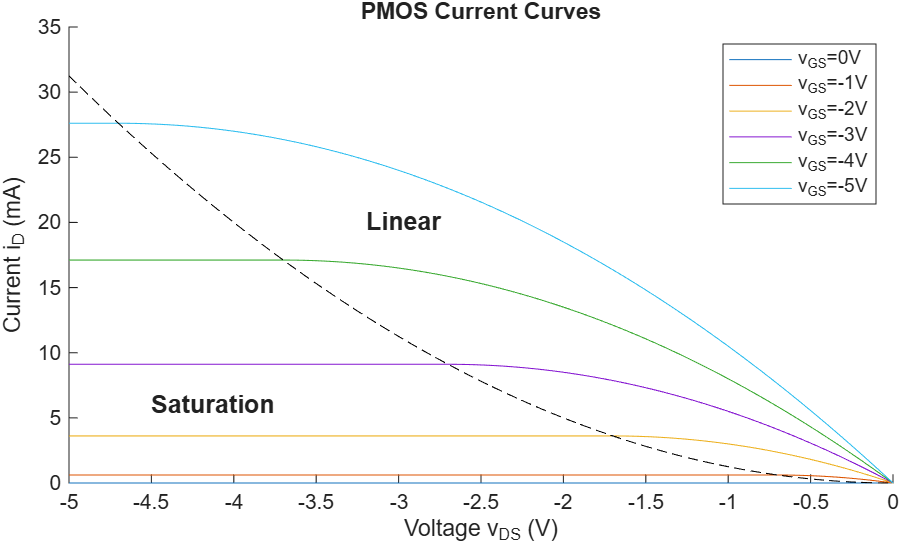
\includegraphics[width=5.64799978127734in]{plot.png}
\end{center}
\end{answer}
\end{partquestion}

\end{mainquestion}
